\subsection{Statistical and sensitivity analysis}
\label{sec:forward}
We now exploit the PC surrogate to study the statistics of the 
water surface elevation, and to quantify its sensitivity to the
uncertain input parameters and thus to anticipate their impact on
the inverse problem.  In doing so, it is emphasized that 
no additional Geoclaw simulations were needed to obtain
the information presented below, rather it is obtained either directly 
from the coefficients of the PC surrogate or by sampling the corresponding
representations for different values of $\xxi$.

Figure~\ref{fig:ave} shows the evolution of
PC mean water surface elevation and its two standard deviations
bounds at the four gauge locations as indicated in each panel.  
The standard deviation is insignificant during the two hours
of the simulations and therefore was not included in the plots.
This standard deviation however increases as the tsunami increase
and its effect approaches the gauge locations. 
To quantity the contribution of each
uncertain parameter to the variance in water surface elevation, we calculate the total sensitivity index 
using the PC coefficients ~\citep{Alexanderian2012,Sudret,Crestaux}. The total sensitivity index
of  each of the uncertain parameters is shown in
Figure~\ref{fig:sens} for the four gauges. The Manning's roughness coefficient
at the shore $N_2$ is clearly dominant and contributes
most to the  water surface elevation variance compared to the other two 
Manning's roughness coefficients;
this is true throughout the simulation time.  The Manning's roughness coefficient
in the ocean $N_{3}$ at gauge number 21419 exhibits small sensitivity index 
the during the second hour of simulation and Manning's roughness coefficient
in the land $N_1$ appears to be an insignificant contributor
to the variance.
\begin{figure}[h]
\begin{tabular}{clc}
        
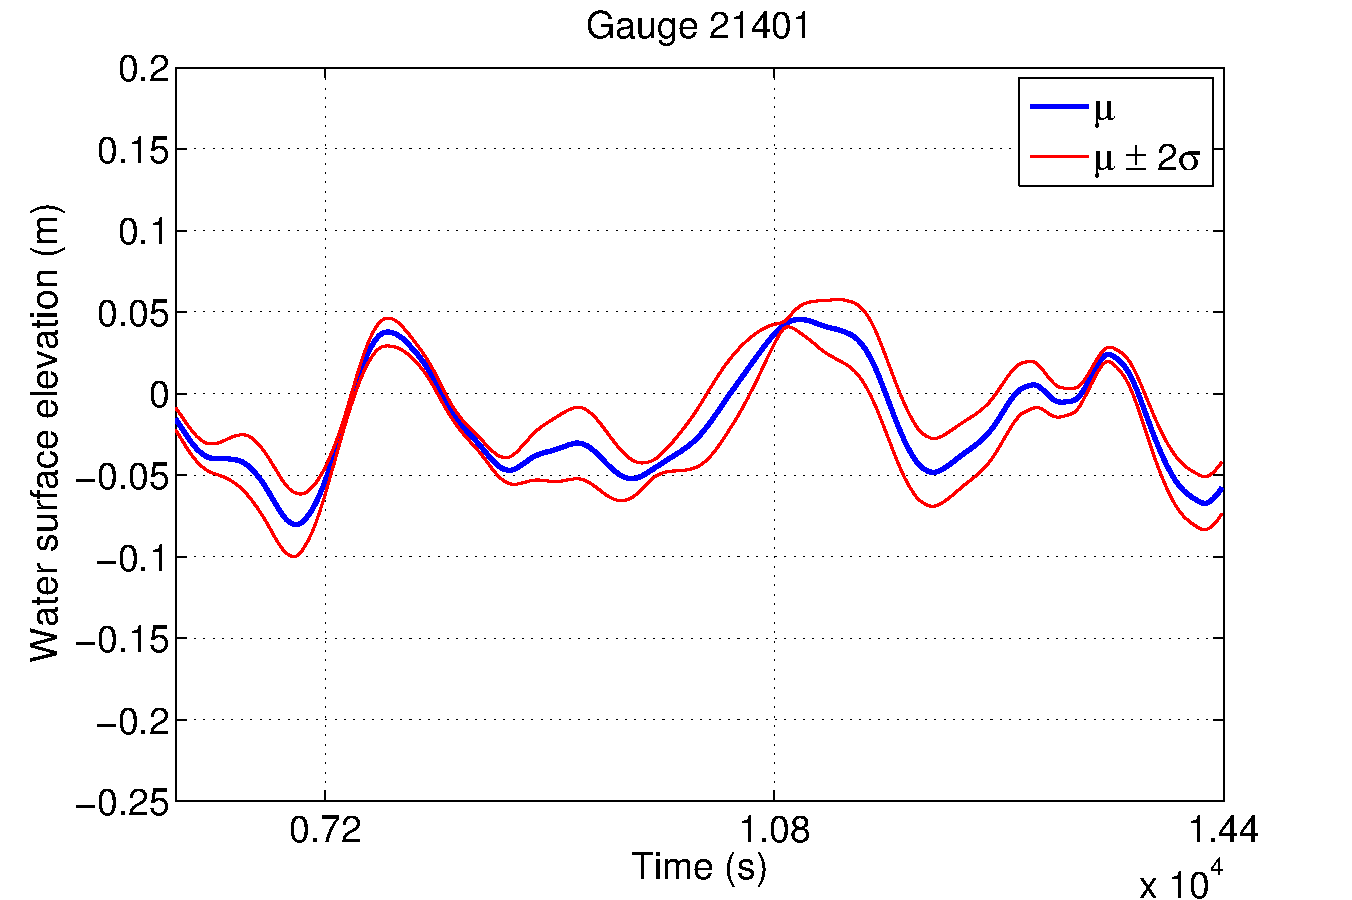
\includegraphics[width=0.475\textwidth]{../figures/musigma1.pdf} &
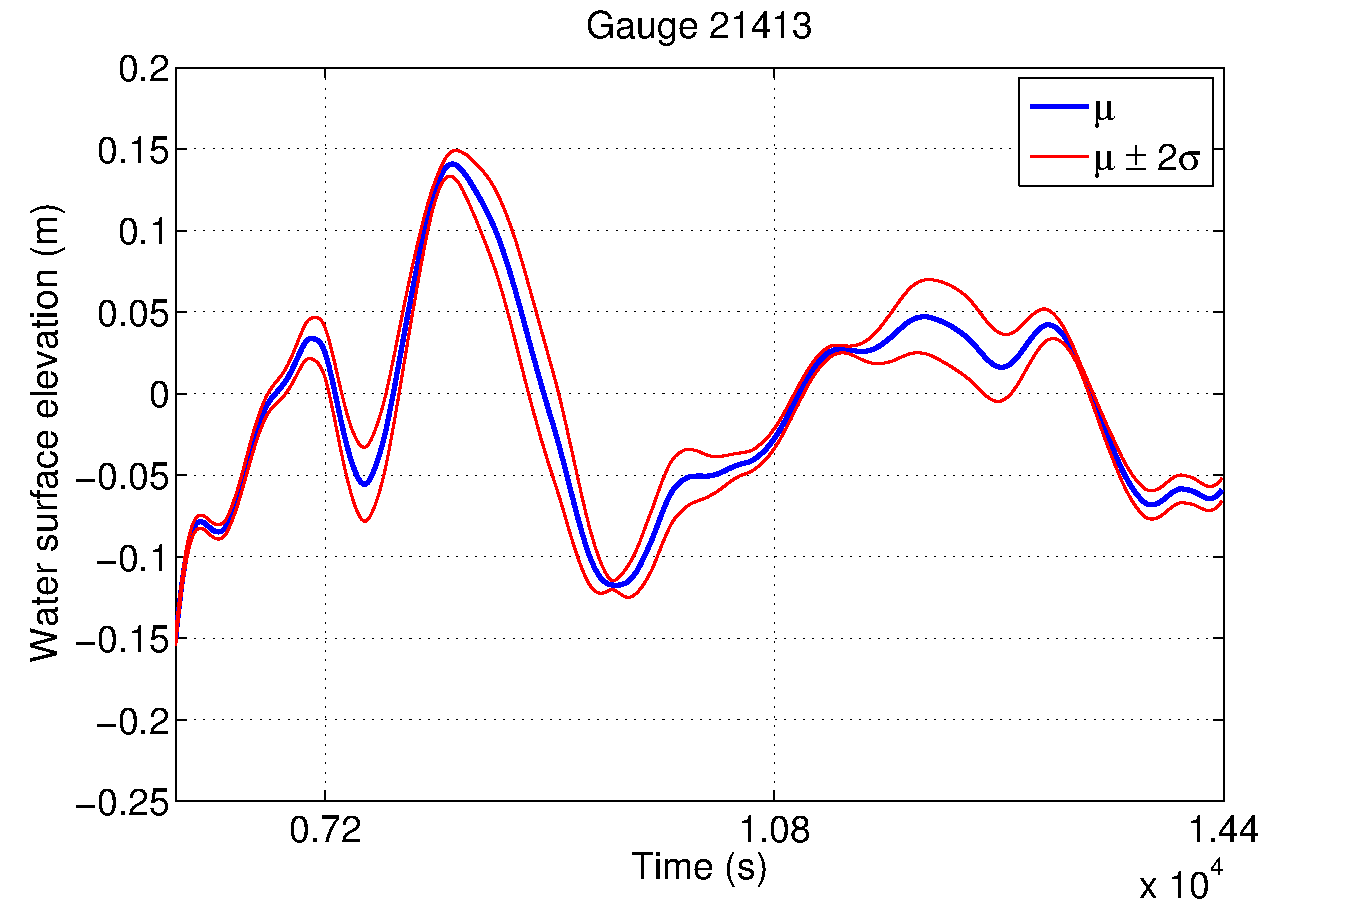
\includegraphics[width=0.475\textwidth]{../figures/musigma2.pdf} \\
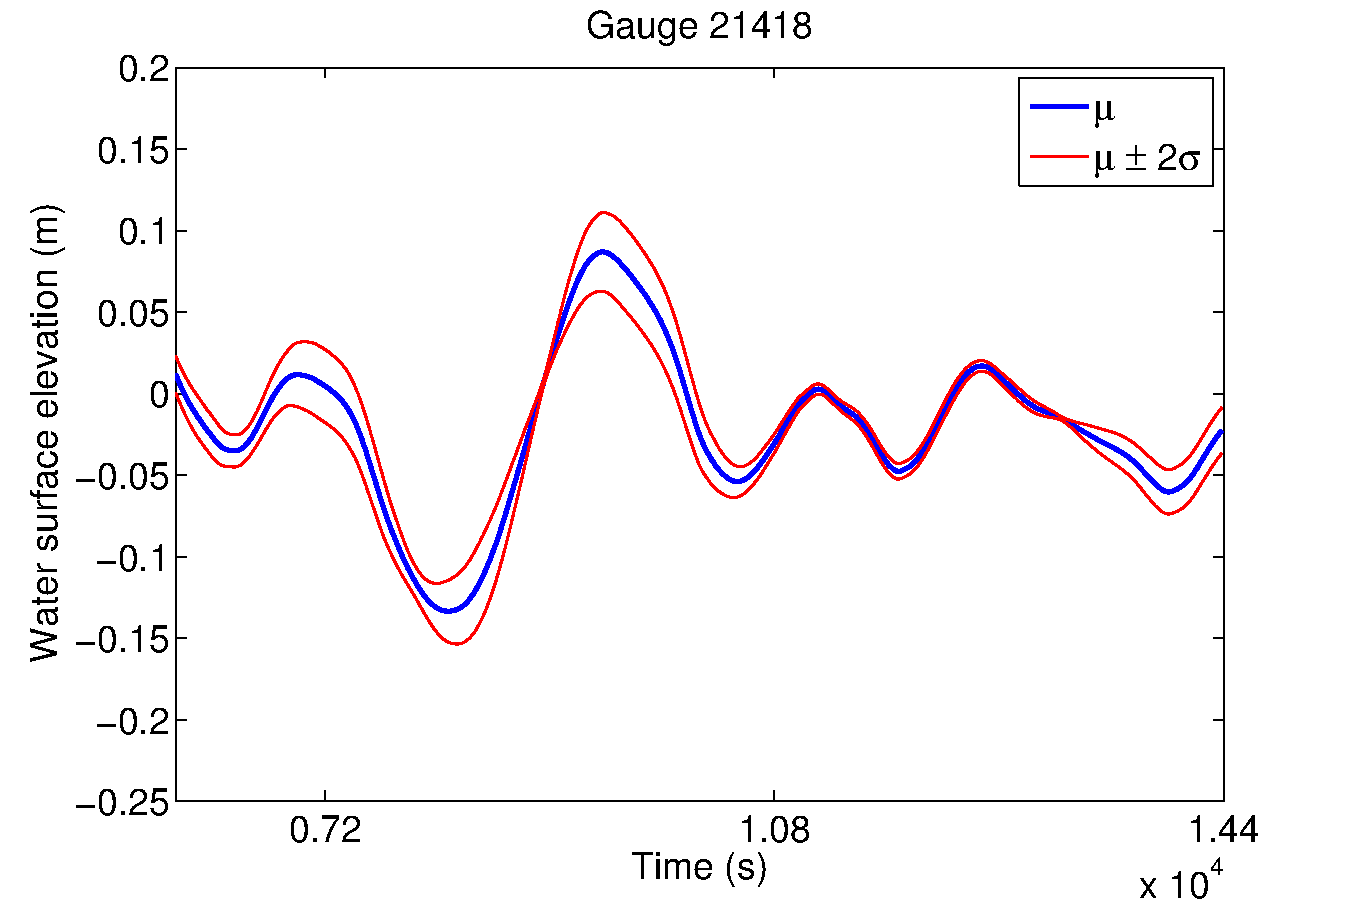
\includegraphics[width=0.475\textwidth]{../figures/musigma3.pdf} &
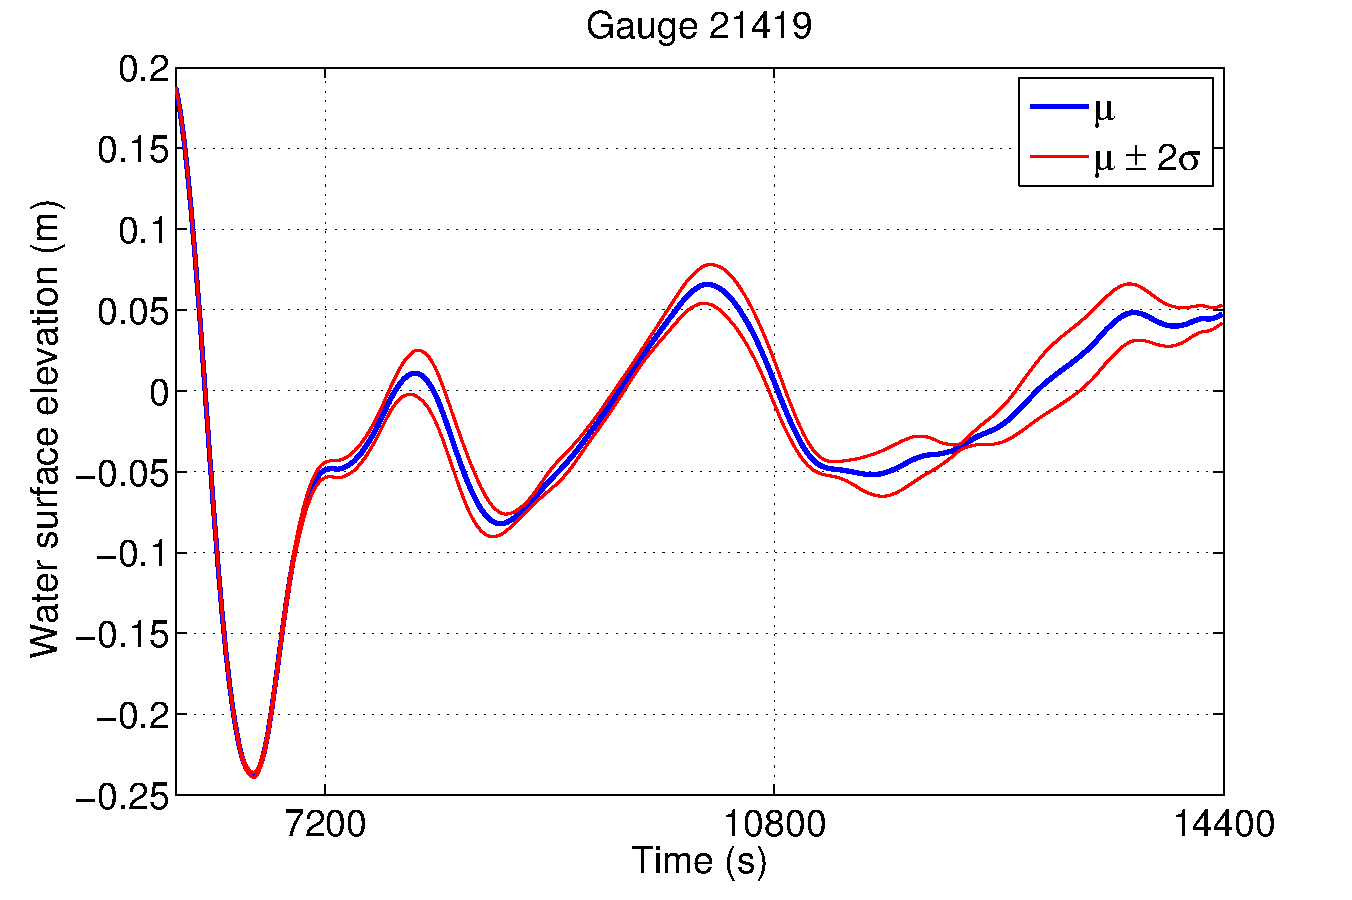
\includegraphics[width=0.475\textwidth]{../figures/musigma4.pdf}
\end{tabular}
\caption{Evolution of PC mean water surface elevation at different gauge locations.}
\label{fig:ave}
\end{figure}
\begin{figure}[h]
\begin{tabular}{clc}
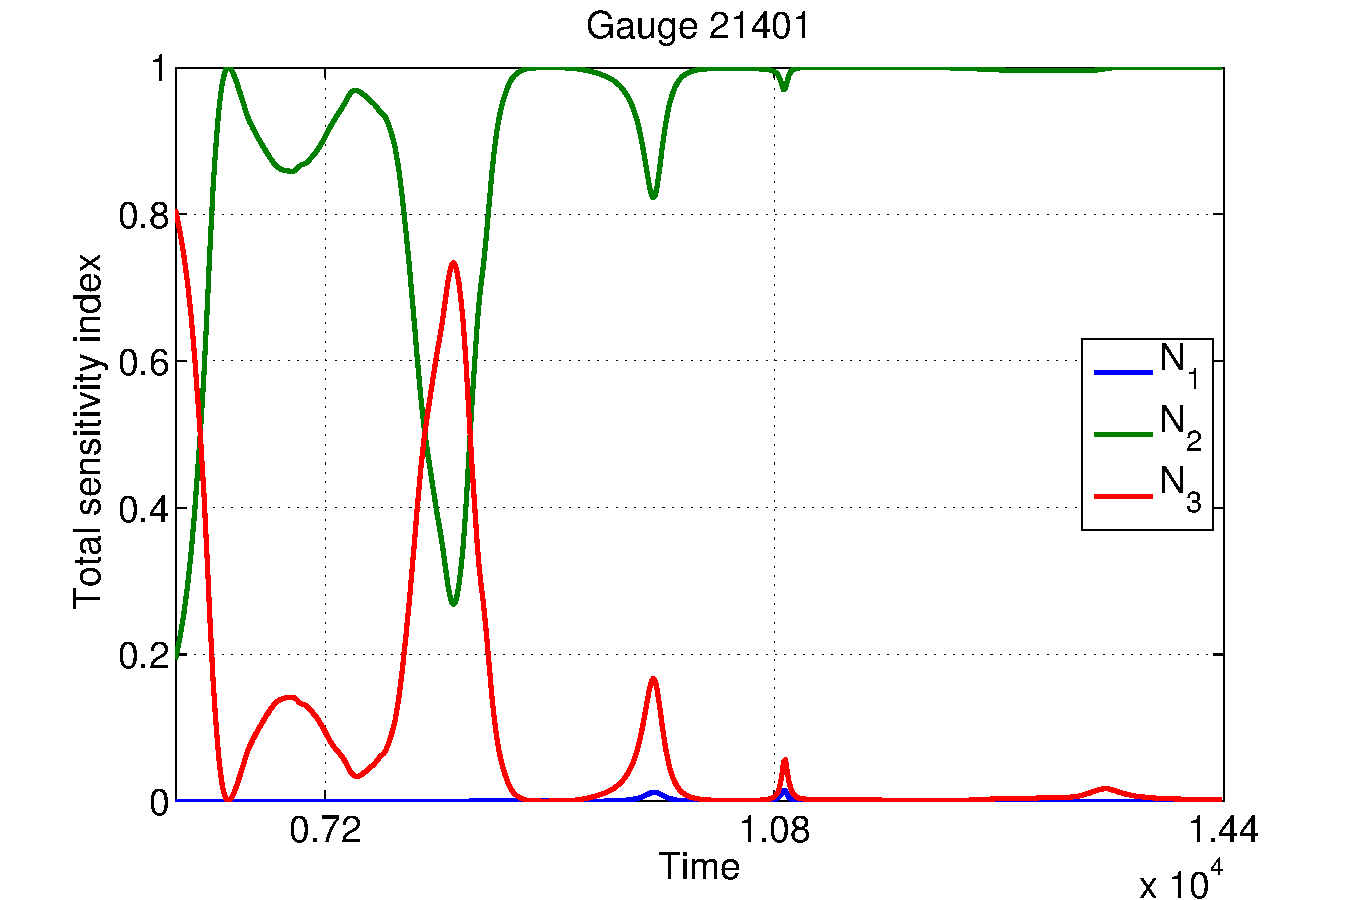
\includegraphics[width=0.475\textwidth]{../figures/sens1.pdf} &
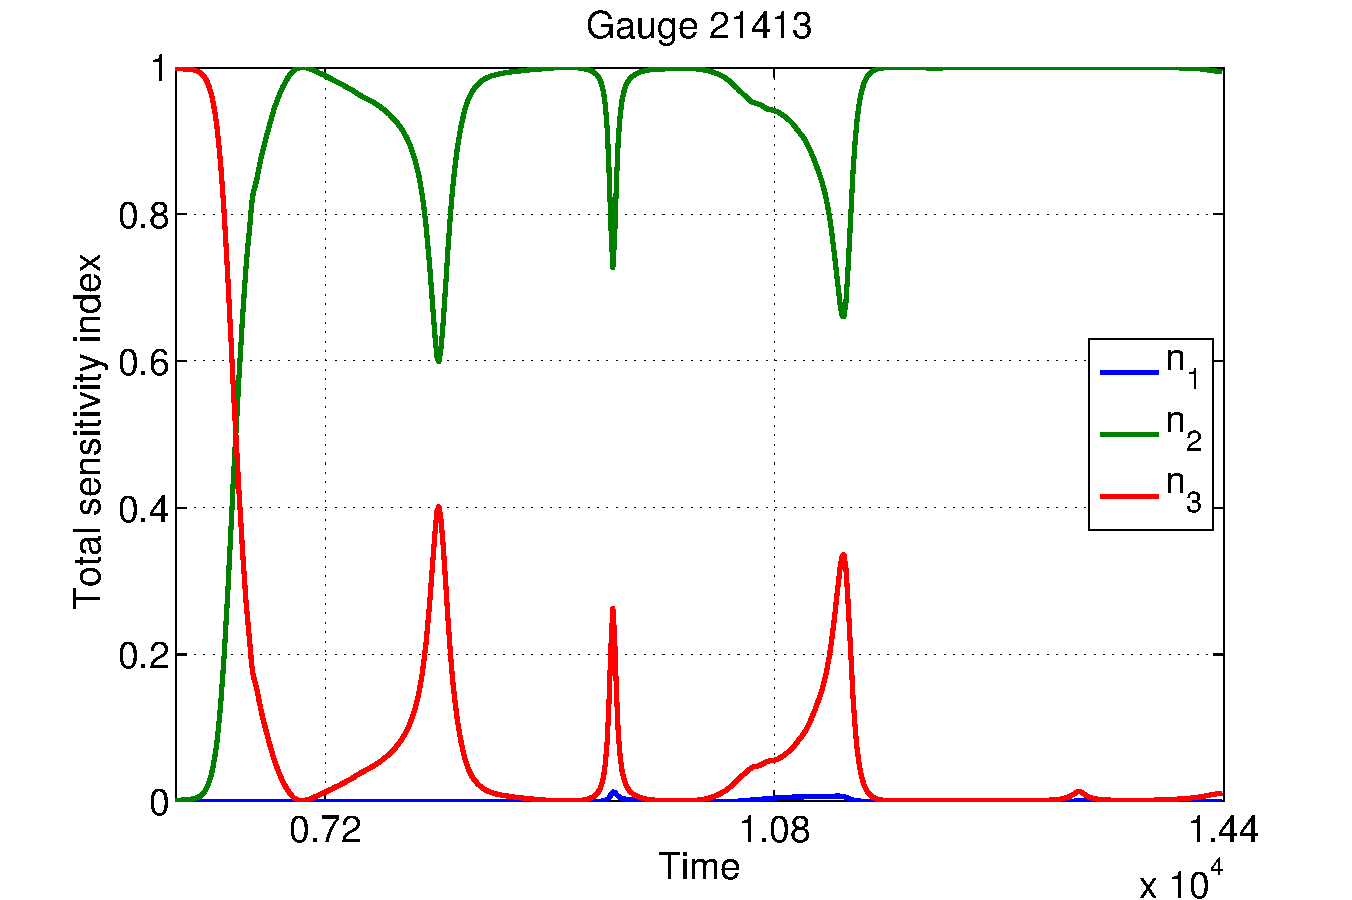
\includegraphics[width=0.475\textwidth]{../figures/sens2.pdf} \\
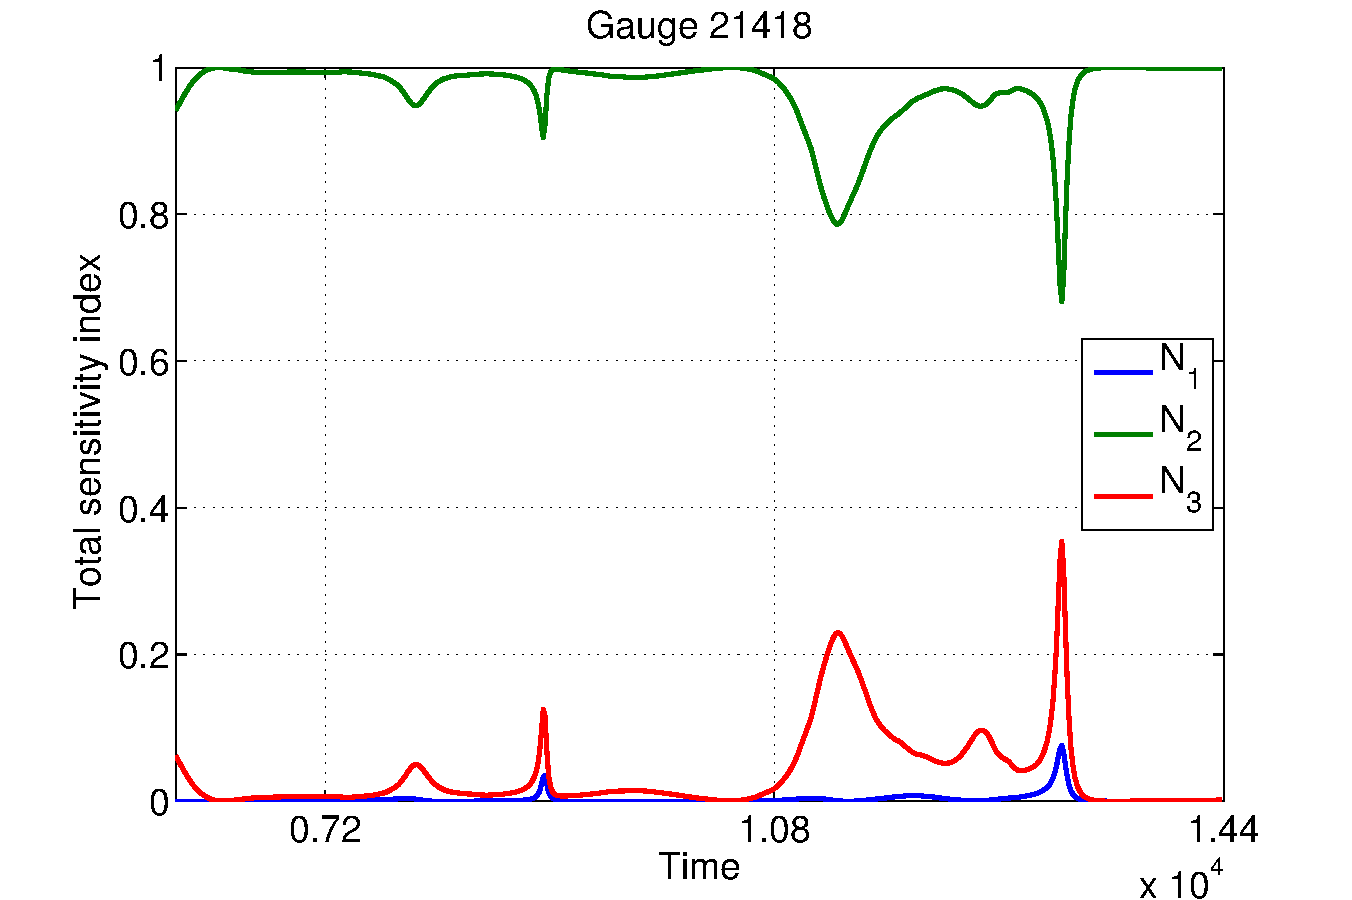
\includegraphics[width=0.475\textwidth]{../figures/sens3.pdf} &
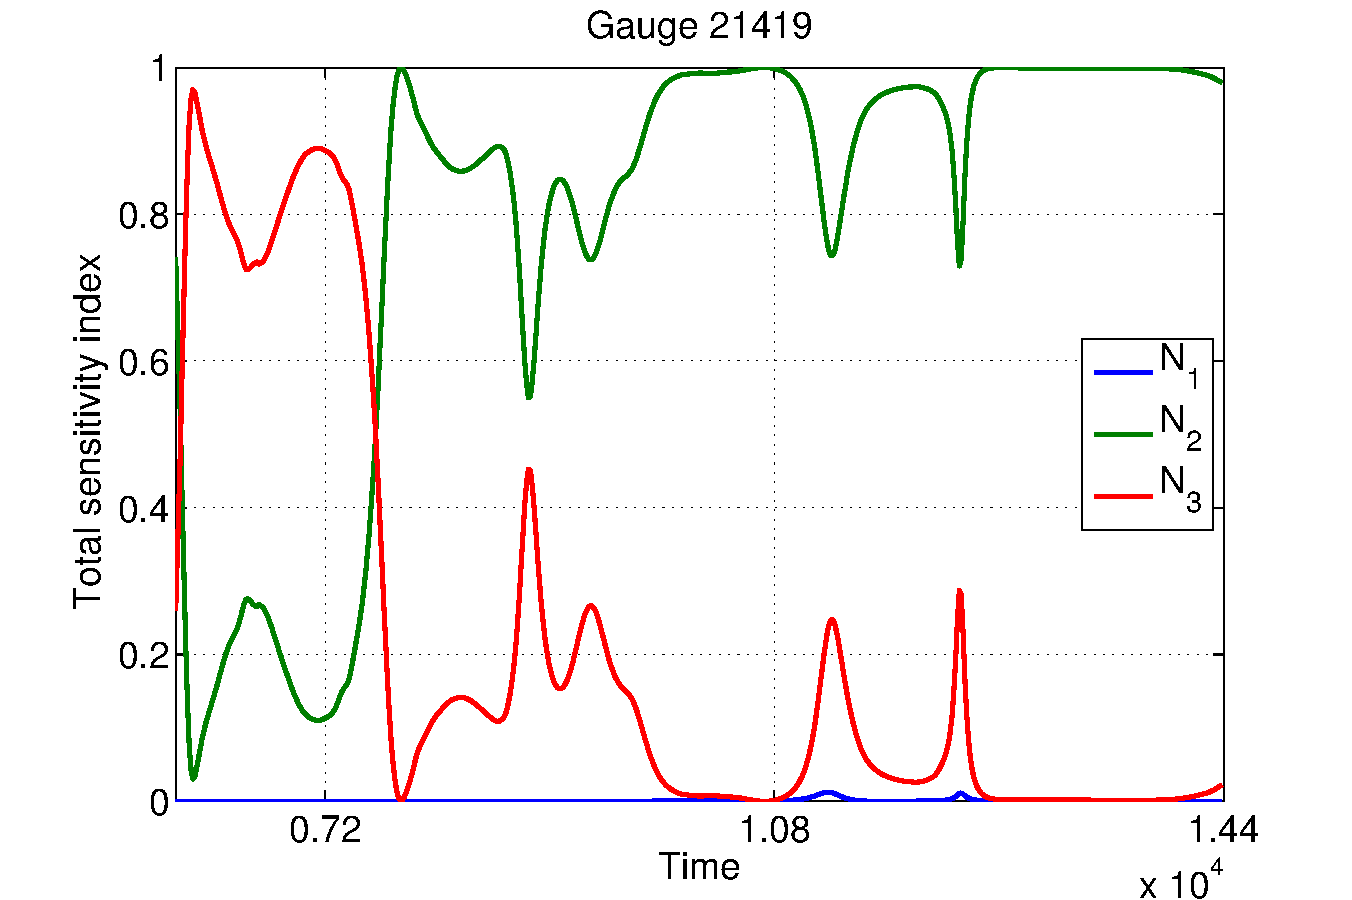
\includegraphics[width=0.475\textwidth]{../figures/sens4.pdf}
\end{tabular}
\caption{Total sensitivity index of different input parameters.}
\label{fig:sens}
\end{figure}


%The impact of $\alpha$ and $V_{max}$ for fixed $m=0$ is illustrated in Figure \ref{fig:response}
%for the area-averaged SST within the $42~km\times42~km$ analysis region; the
%different panels illustrate the time evolution of the SST response
%surfaces. Their most striking features are the relatively flat
%horizontal contours on Sep~17 and Sep~18 indicating that SST depends
%only mildly on $V_{\max}$ even during peak winds;
% unsurprisingly these contours turn completely flat on Sep
%19 (and afterwards) when the winds dip below 10~m/s. The multiplicative
%factor $\alpha$, however, exerts a strong influence on SST even
%under mild wind conditions.  This influence is relatively
%weak for the low $\alpha$ range and increases substantially for the
%higher $\alpha$ as evidenced by the packed contours.  The temperature
%response surfaces at 50-m and 200-m depths (not shown) exhibit
%roughly the same structure as the surface, with milder
%dependence on $V_{\max}$ even during the peak winds of Sep~18.

The same statistical analysis can be performed for the
entire domain in 2D. Figure~\ref{fig:mean2d}(top row) shows
the PC mean water surface elevation for the considered computational
domain at three different times as indicated in the title of each panel.
The standard deviation is also shown in Figure~\ref{fig:mean2d}(bottom row).
\begin{figure}[h]
        \begin{tabular}{ccc}
\hspace*{-65pt}
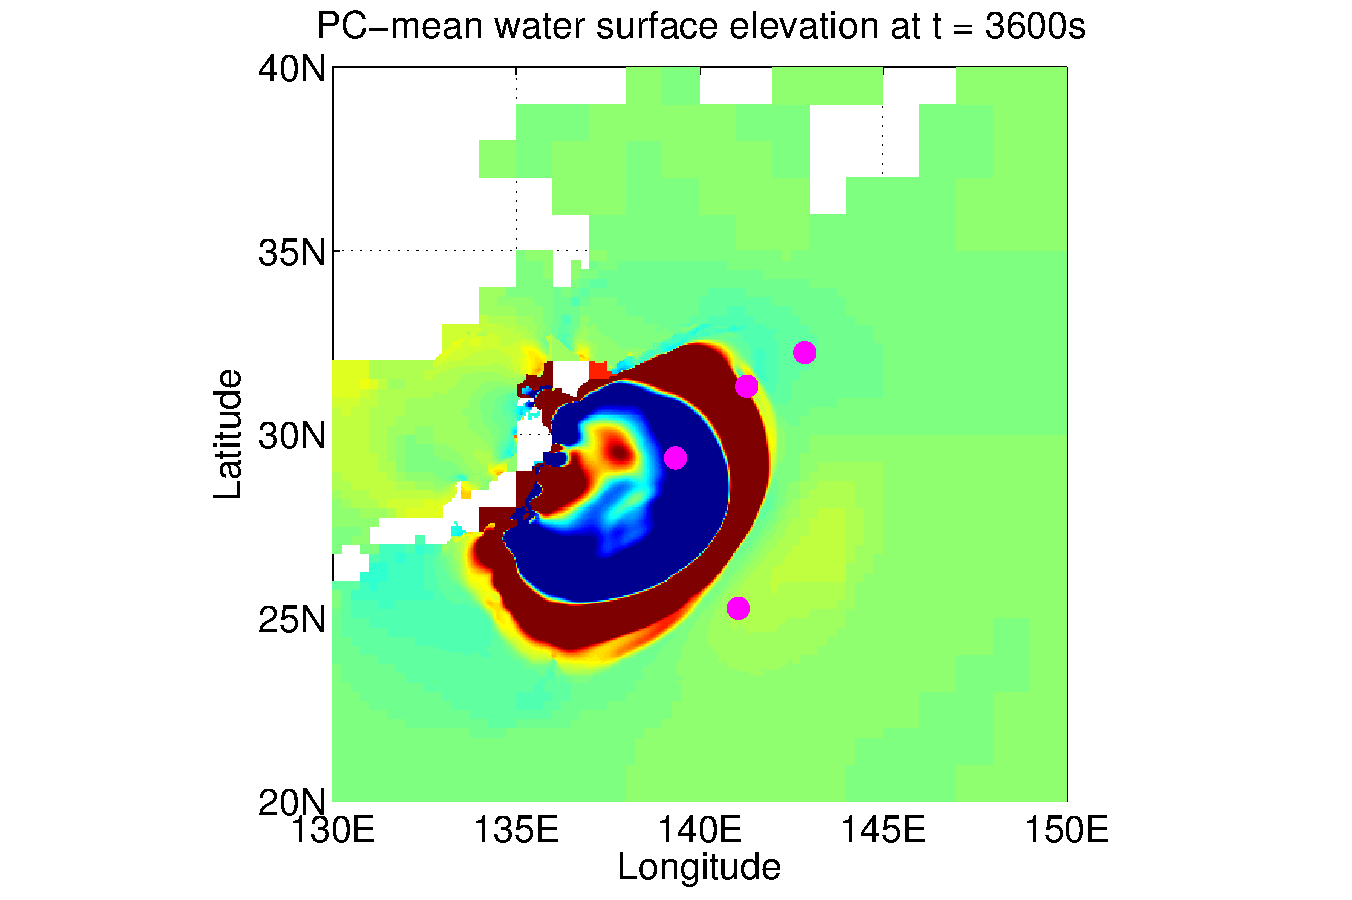
\includegraphics[width=0.45\textwidth]{../figures/mean2d1.pdf} &
\hspace*{-65pt}
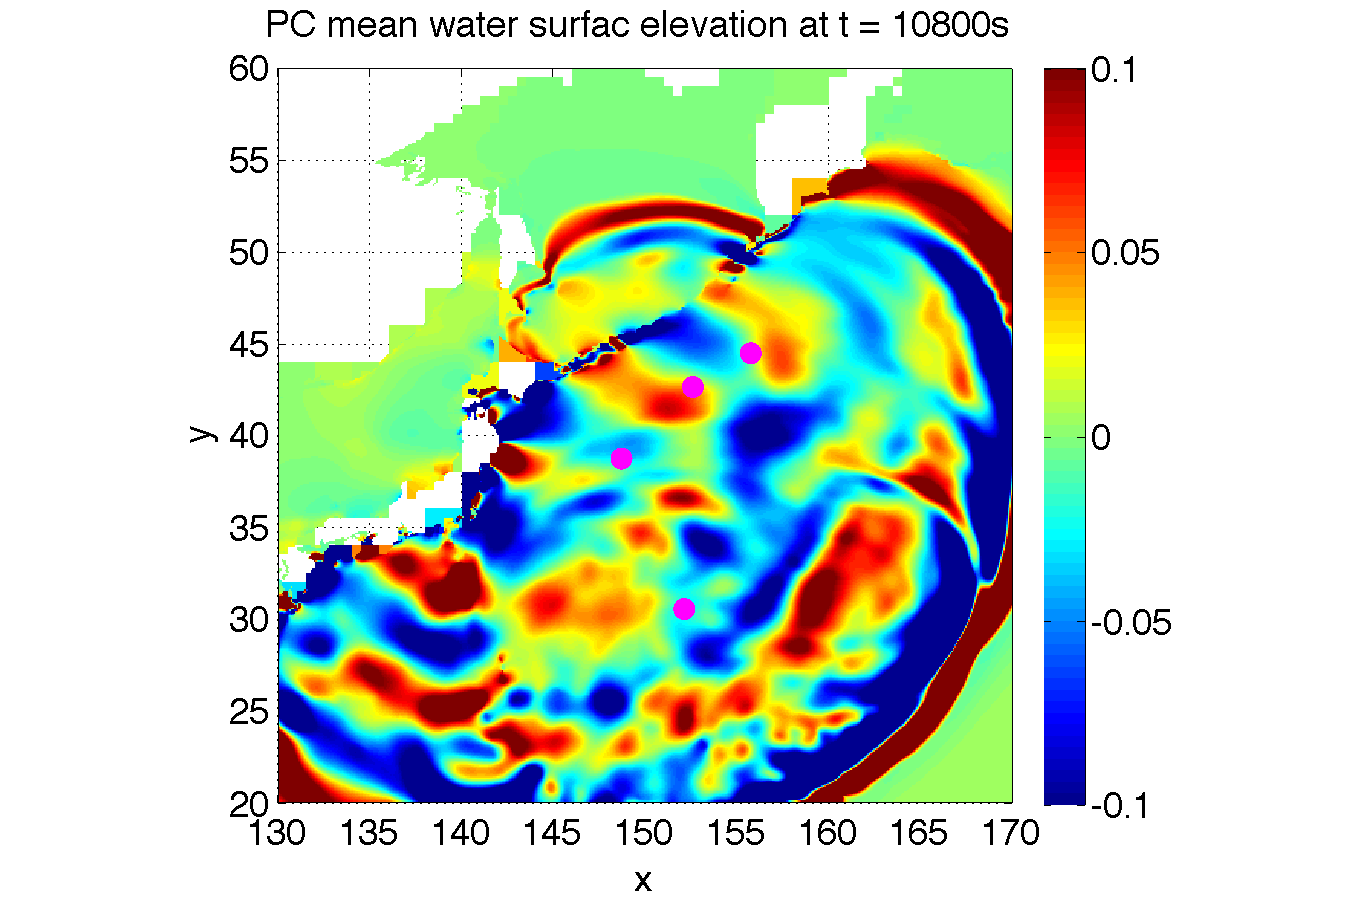
\includegraphics[width=0.45\textwidth]{../figures/mean2d3.pdf} &
\hspace*{-65pt}
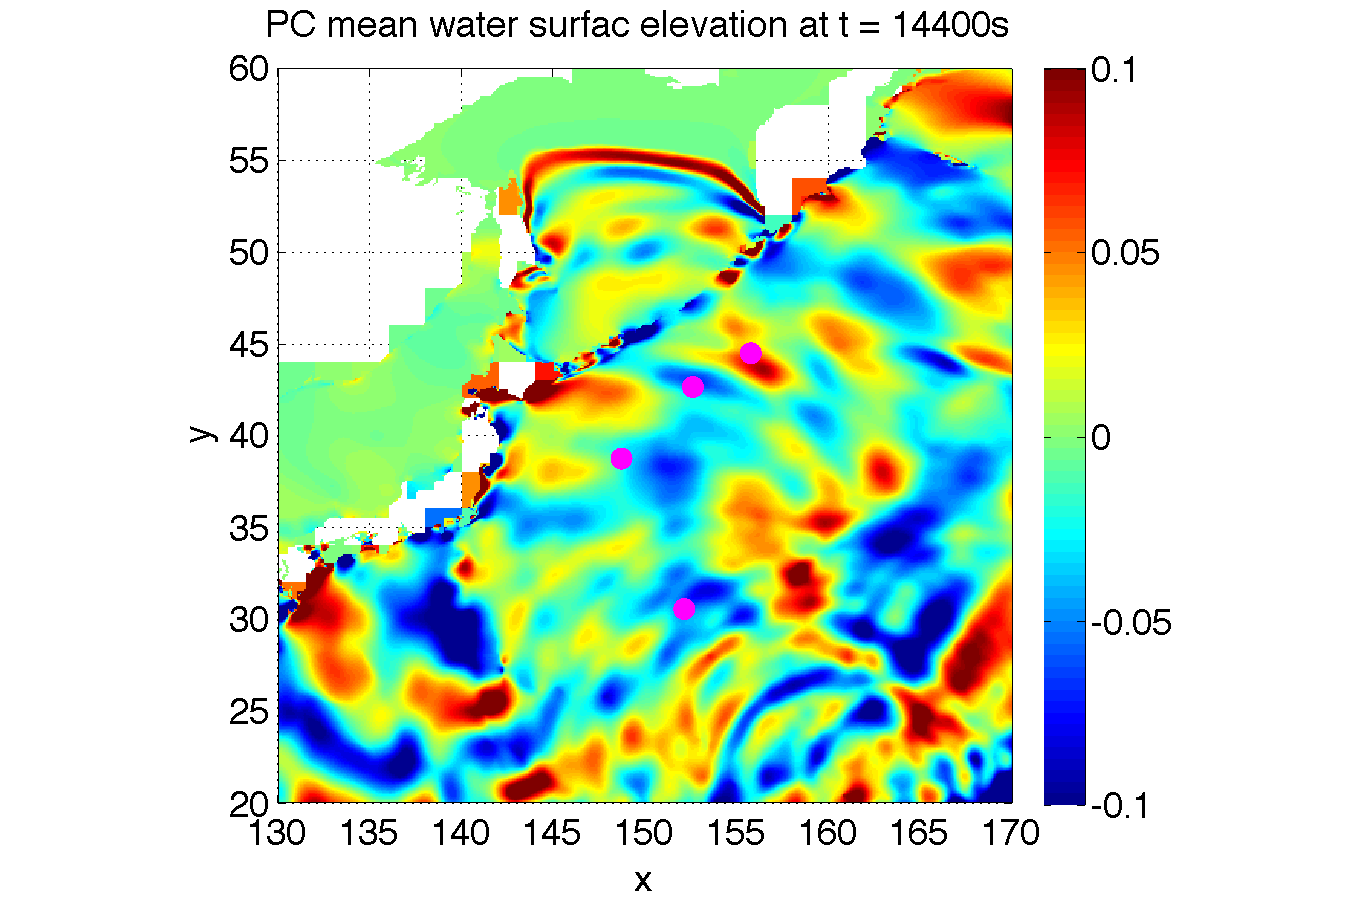
\includegraphics[width=0.45\textwidth]{../figures/mean2d4.pdf} \\
\hspace*{-65pt}
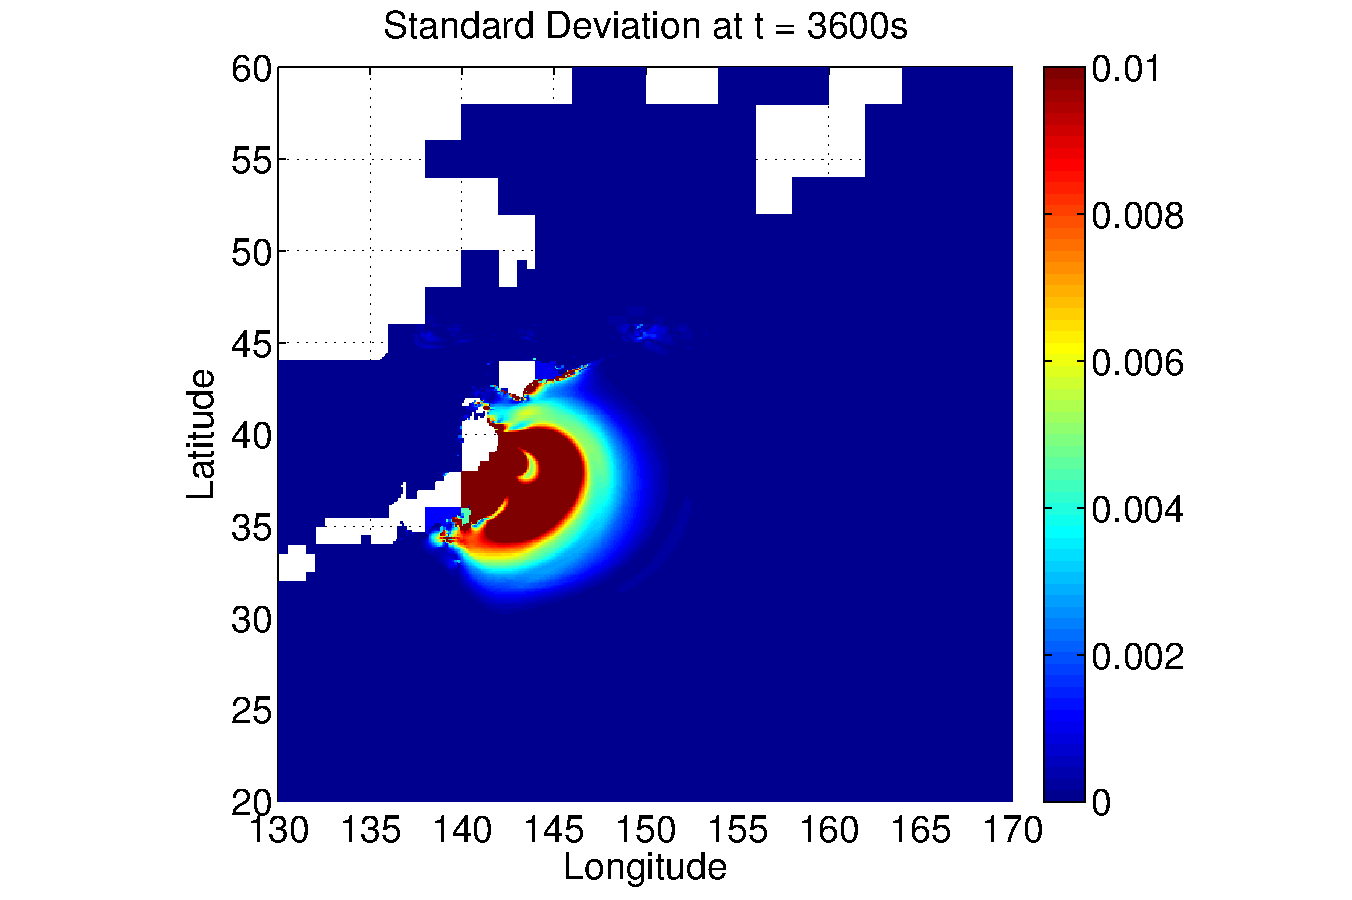
\includegraphics[width=0.45\textwidth]{../figures/sigma2d1.pdf} &
\hspace*{-65pt}
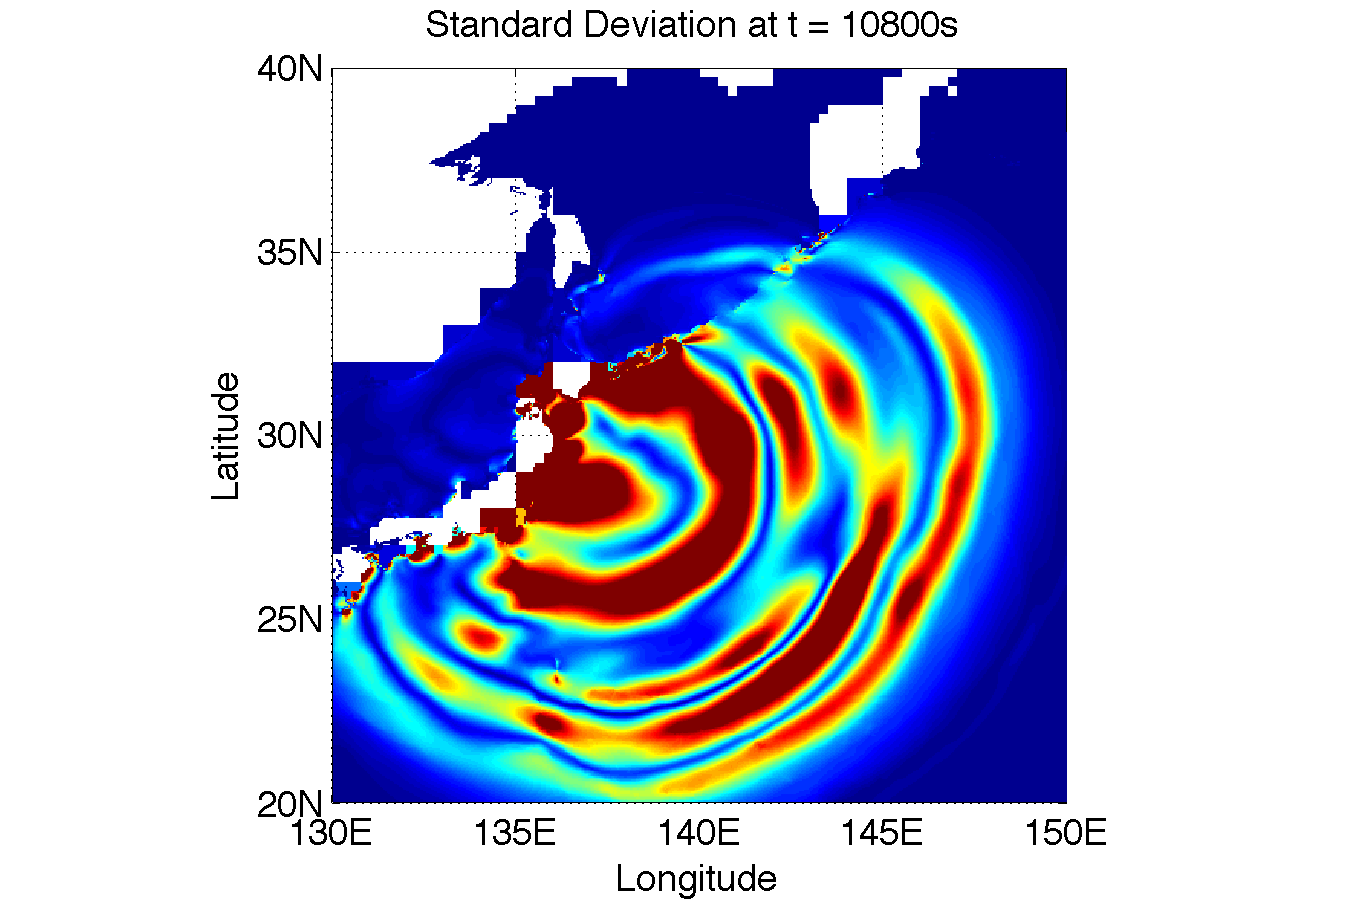
\includegraphics[width=0.45\textwidth]{../figures/sigma2d3.pdf} &
\hspace*{-65pt}
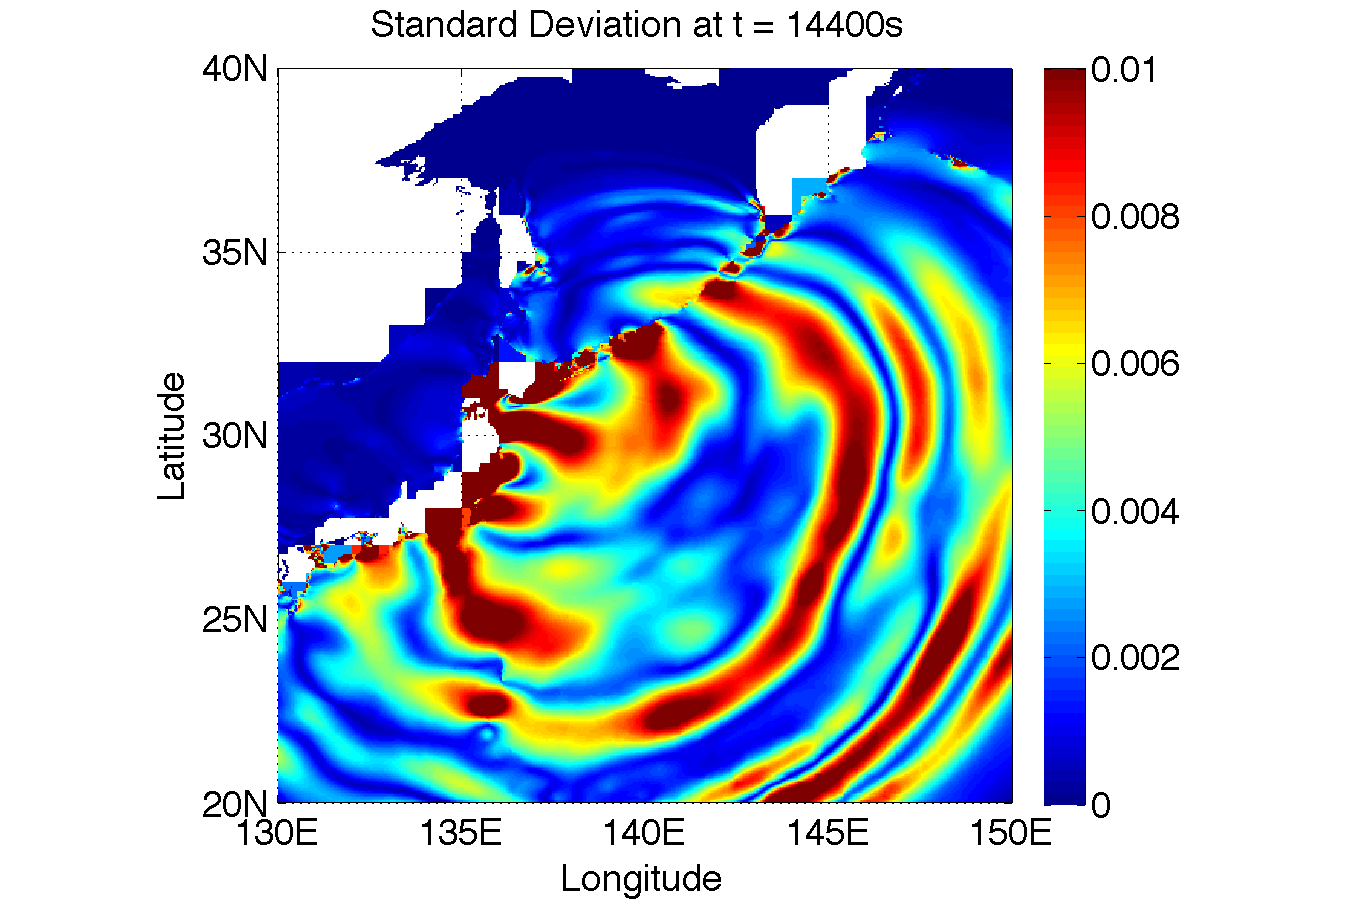
\includegraphics[width=0.45\textwidth]{../figures/sigma2d4.pdf}
\end{tabular}
\caption{PC mean (top row) and standard deviation (bottom row) of the water surface elevation at different times.}
\label{fig:mean2d}
\end{figure}
      
\begin{figure}[h]
\begin{tabular}{clc}
 \hspace*{-65pt}
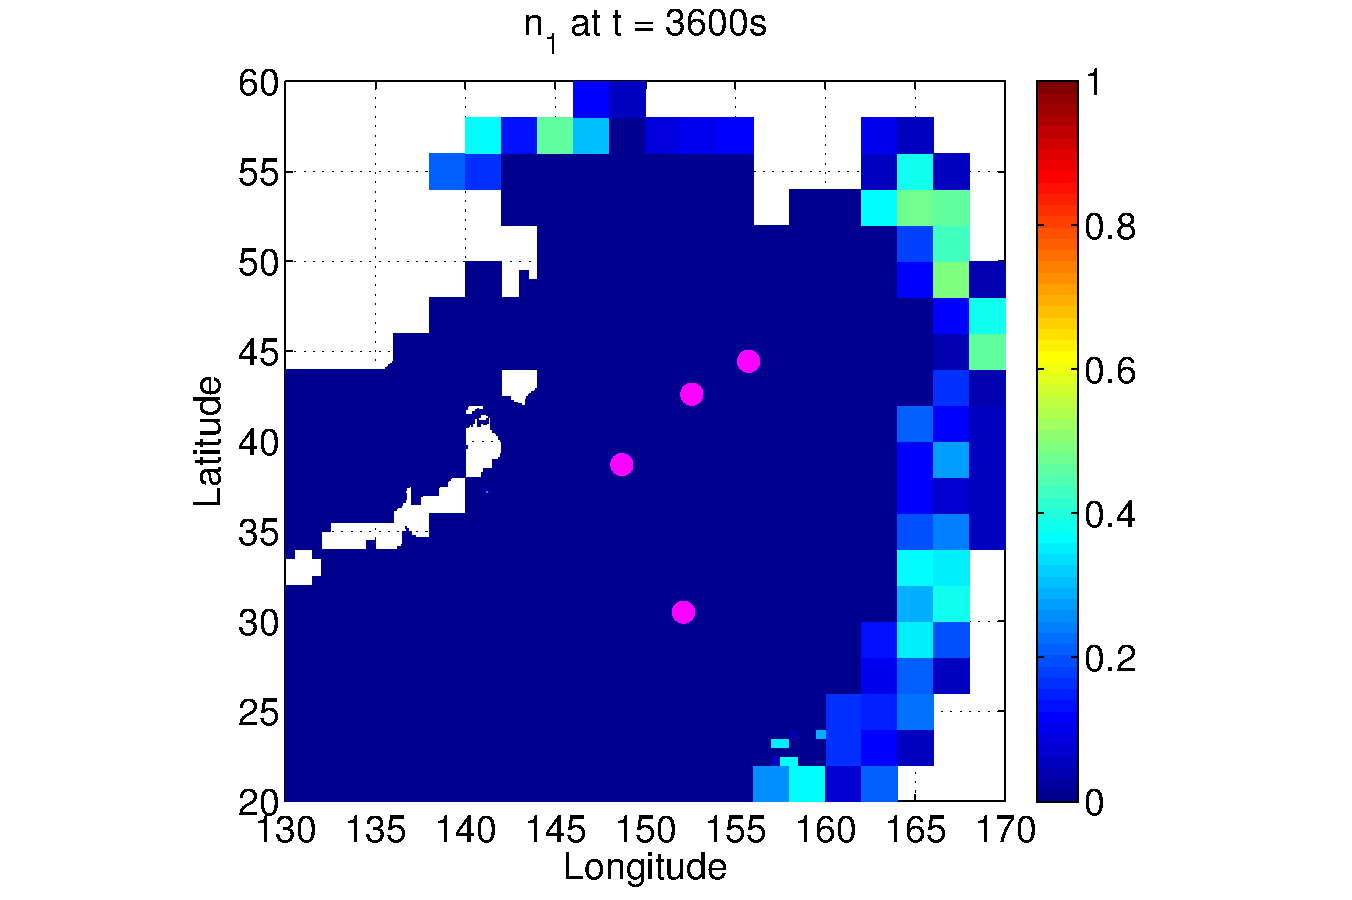
\includegraphics[width=0.45\textwidth]{../figures/T12d1.pdf} &
\hspace*{-65pt}
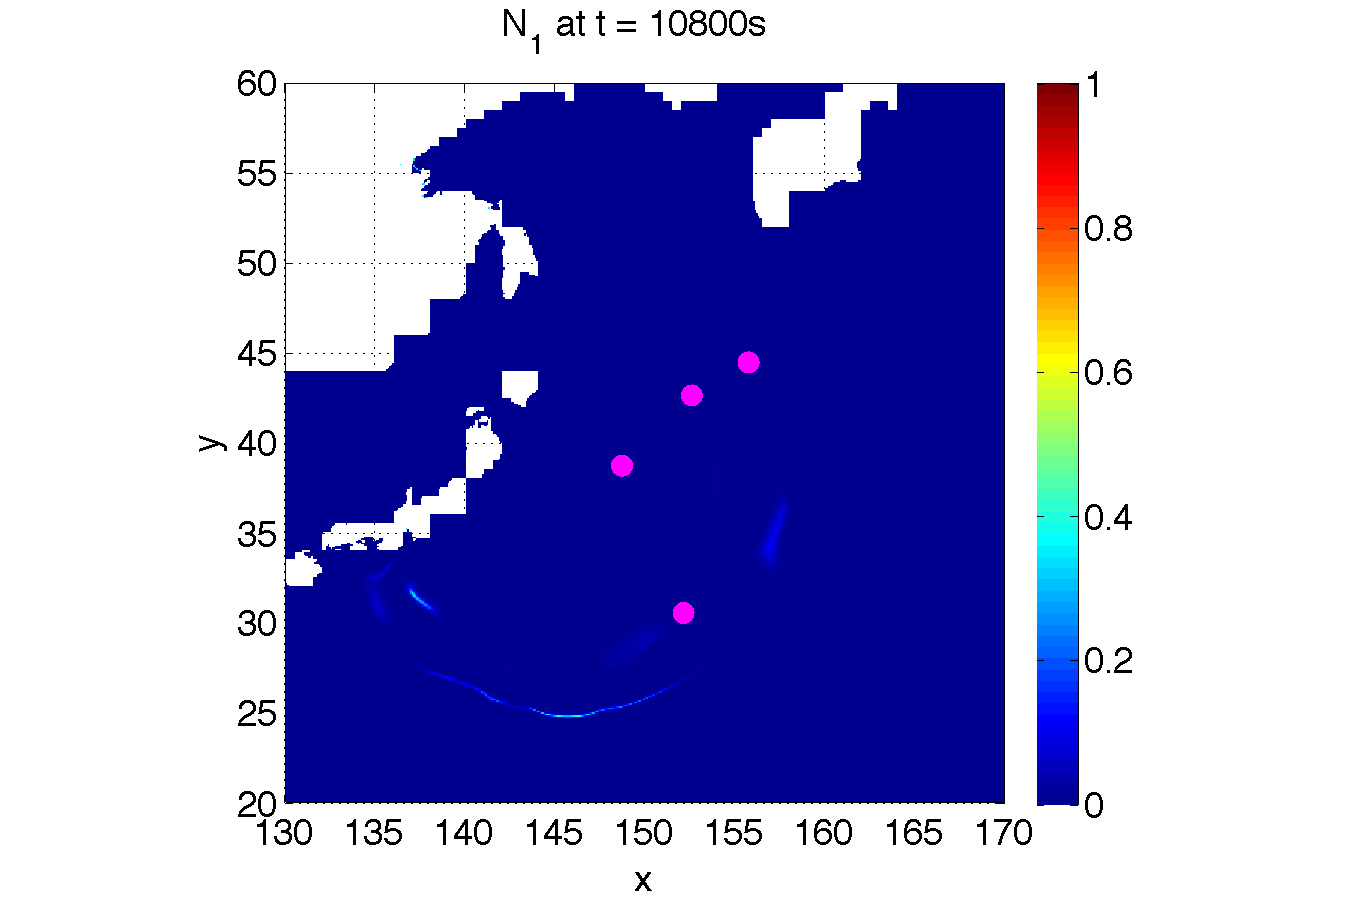
\includegraphics[width=0.45\textwidth]{../figures/T12d3.pdf} &
\hspace*{-65pt}
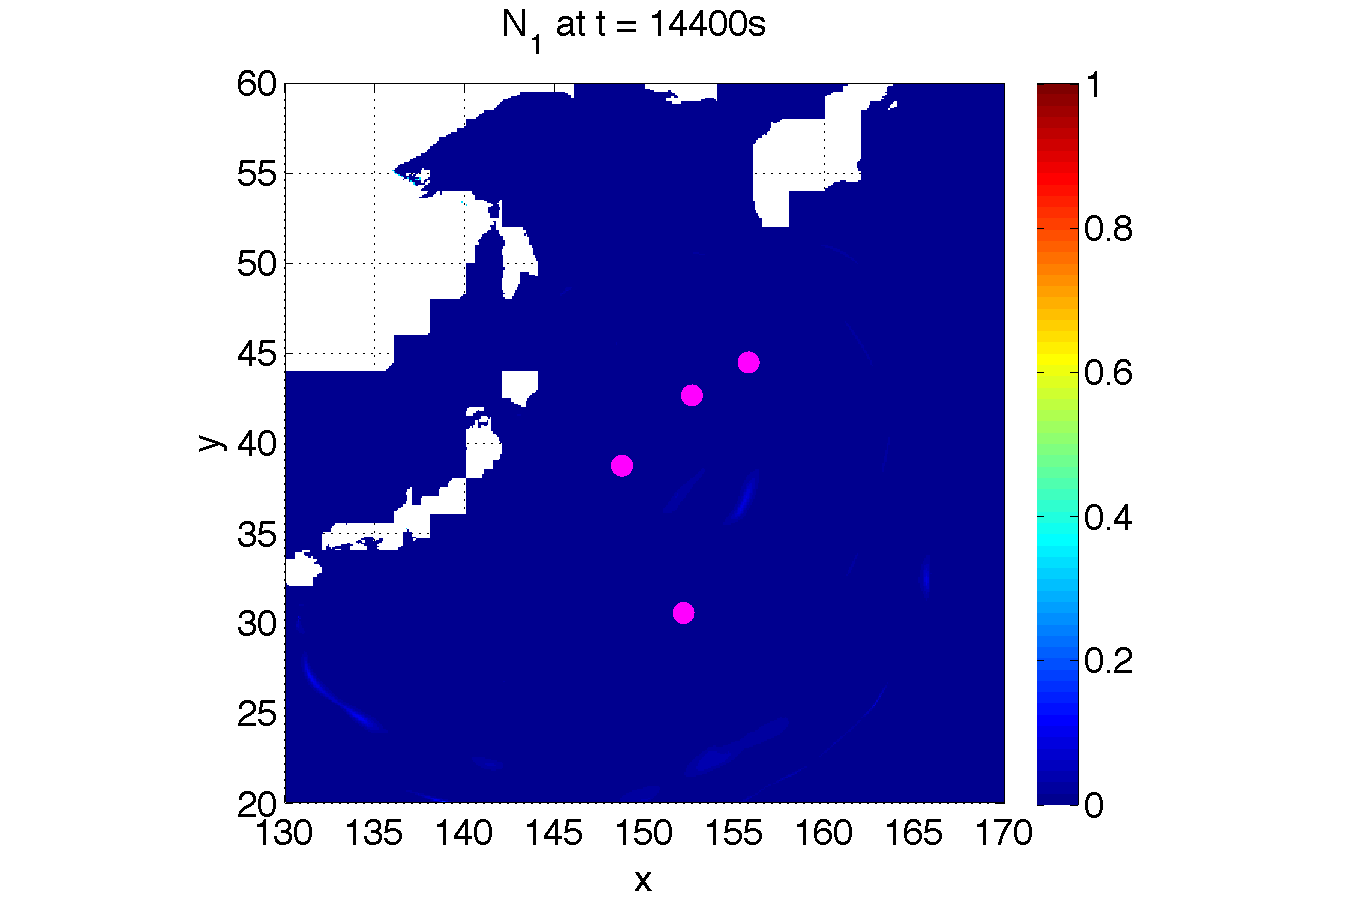
\includegraphics[width=0.45\textwidth]{../figures/T12d4.pdf} \\
\hspace*{-65pt}
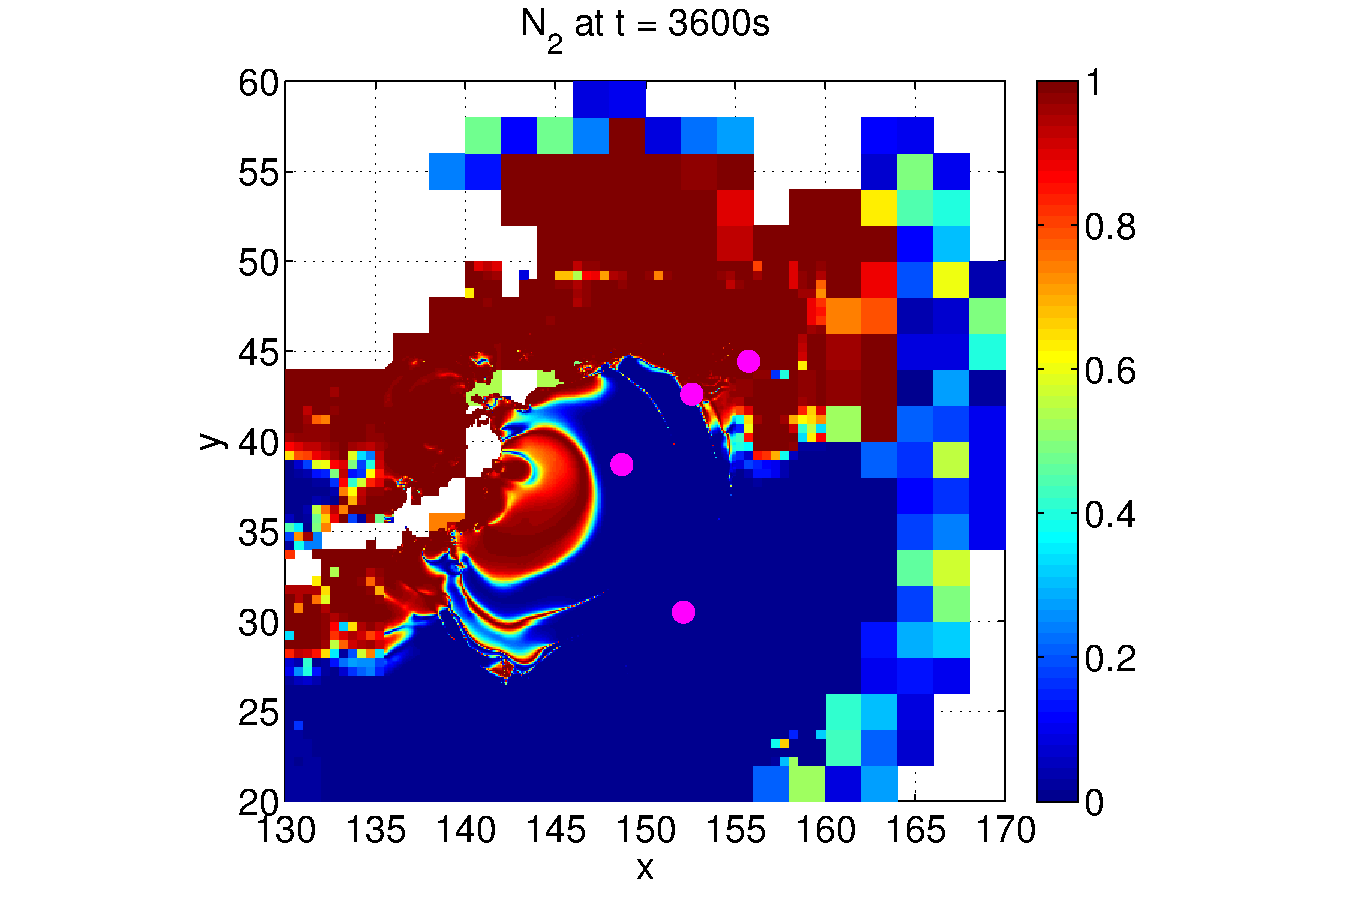
\includegraphics[width=0.45\textwidth]{../figures/T22d1.pdf} &
\hspace*{-65pt}
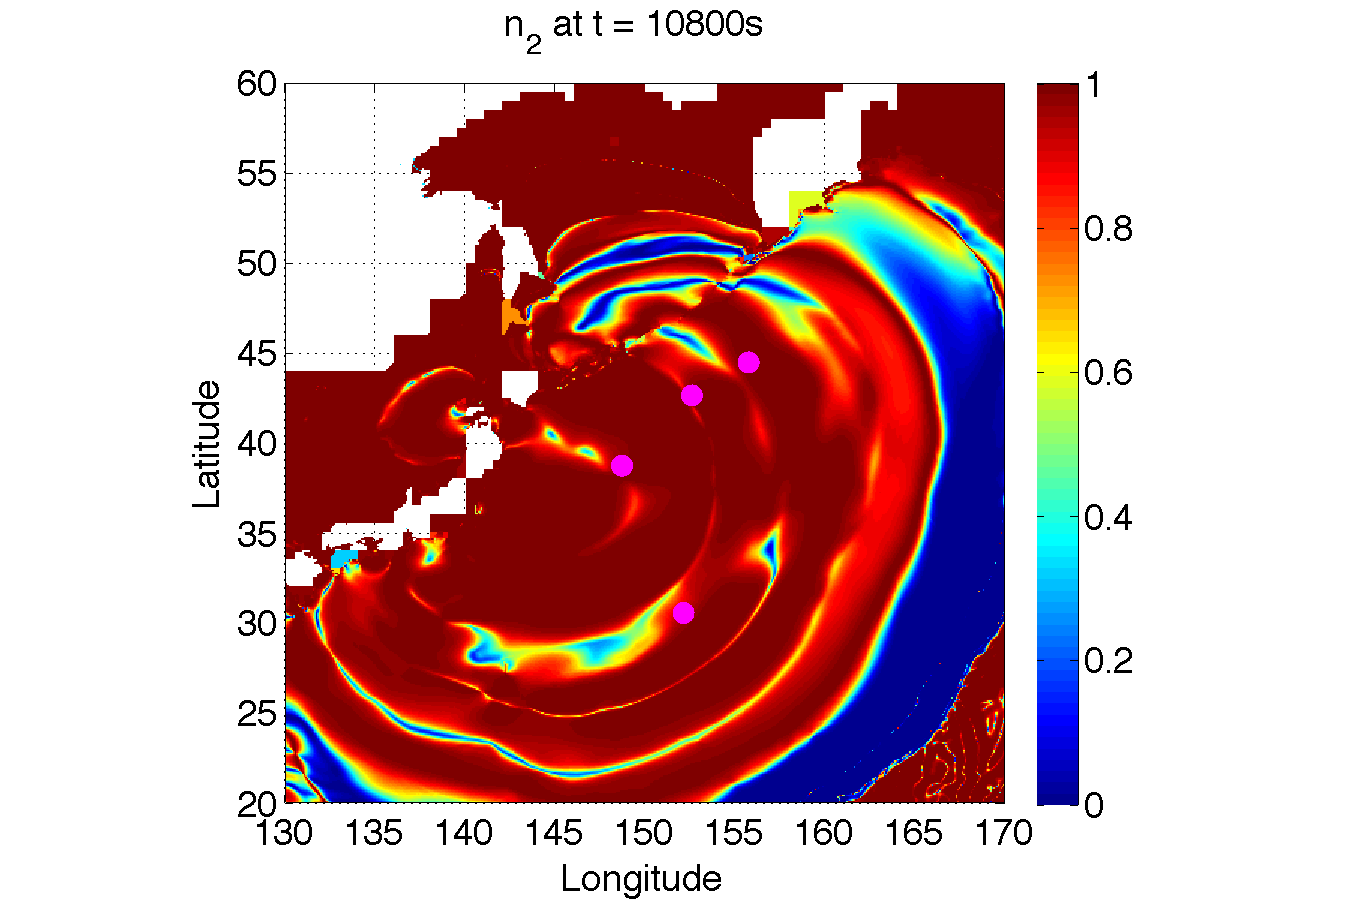
\includegraphics[width=0.45\textwidth]{../figures/T22d3.pdf} &
\hspace*{-65pt}
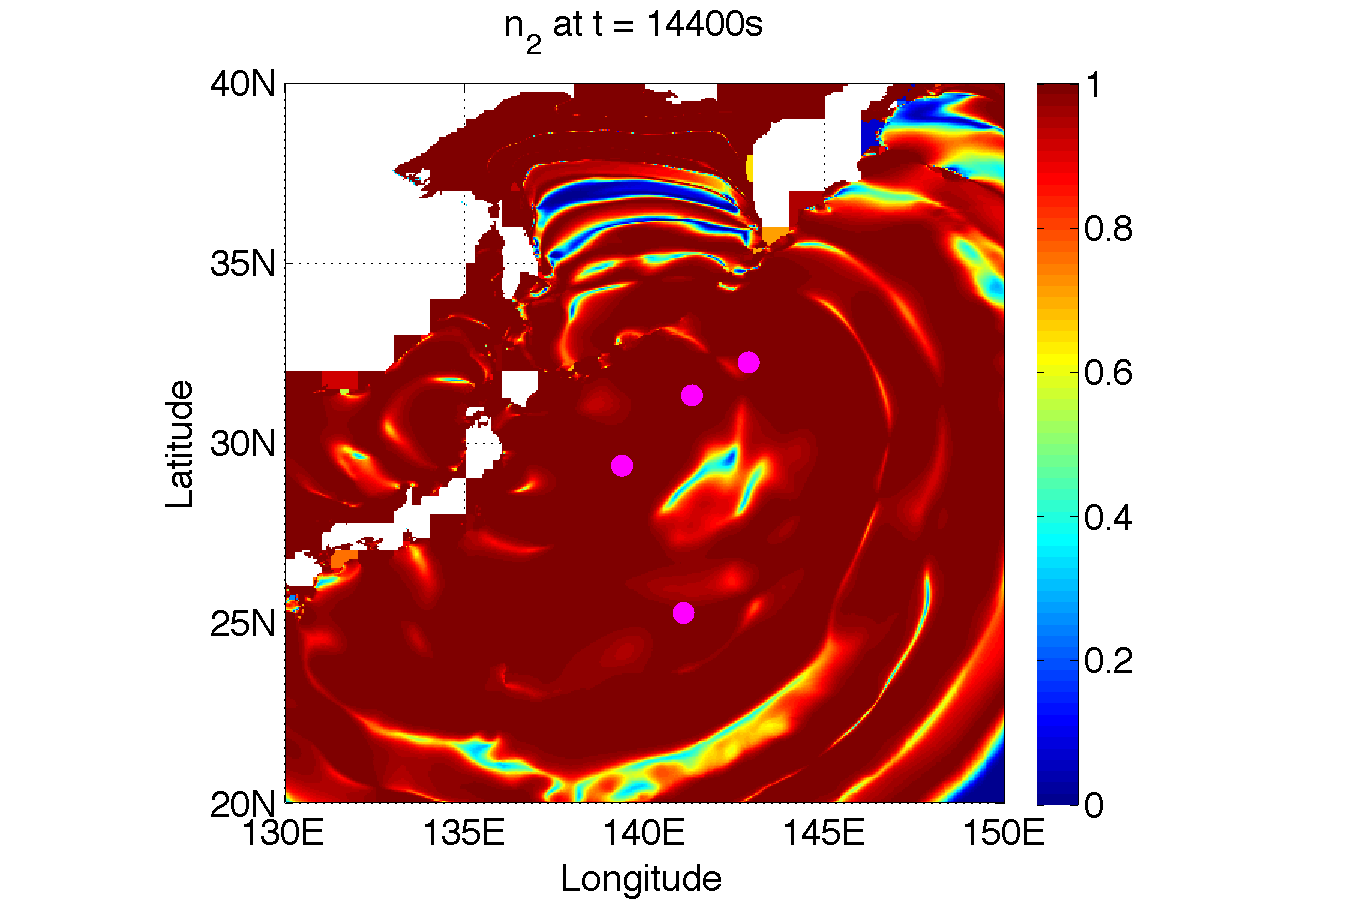
\includegraphics[width=0.45\textwidth]{../figures/T22d4.pdf} \\
\hspace*{-65pt}
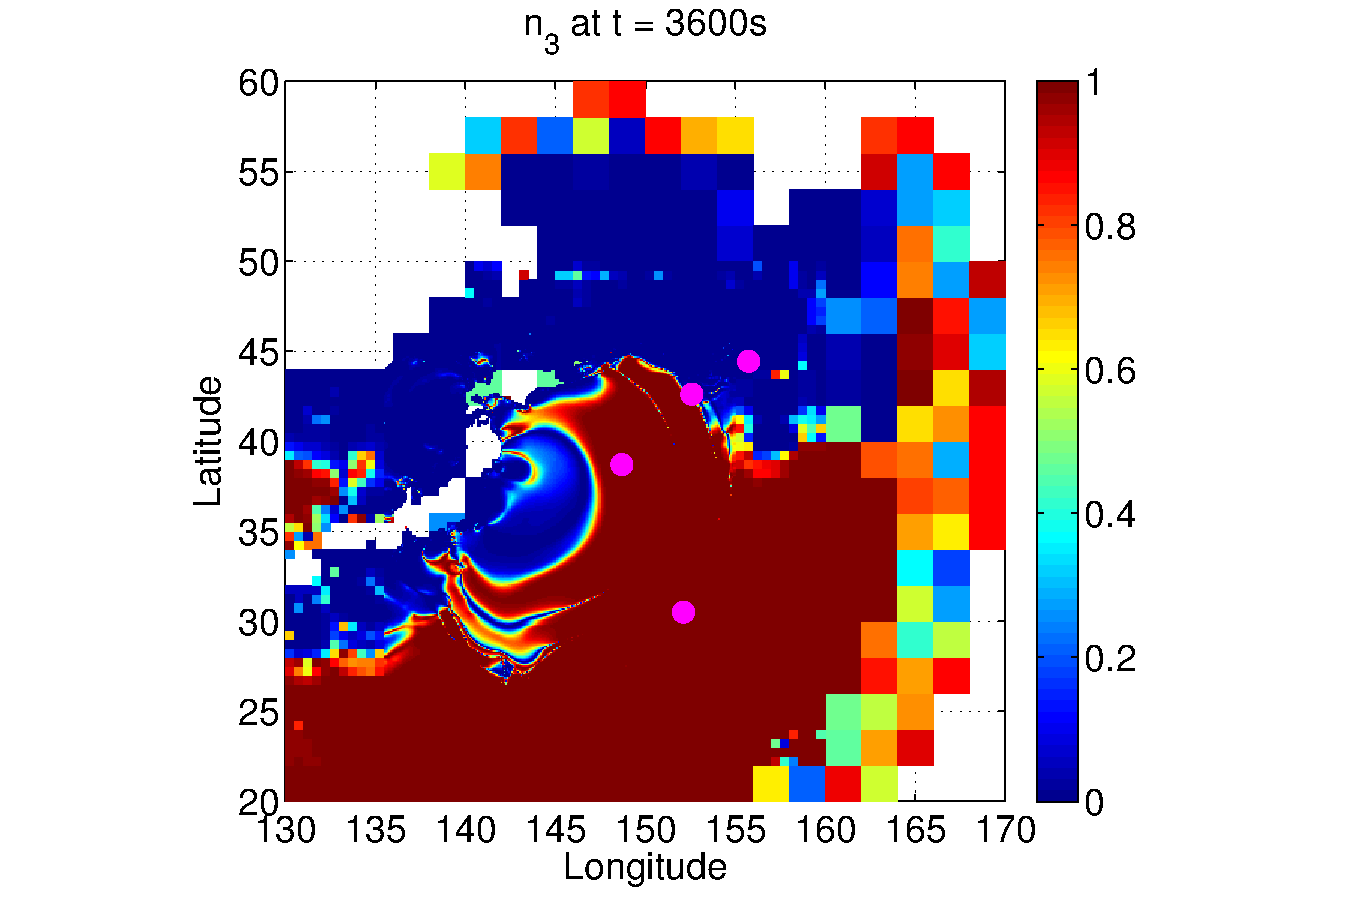
\includegraphics[width=0.45\textwidth]{../figures/T32d1.pdf} &
\hspace*{-65pt}
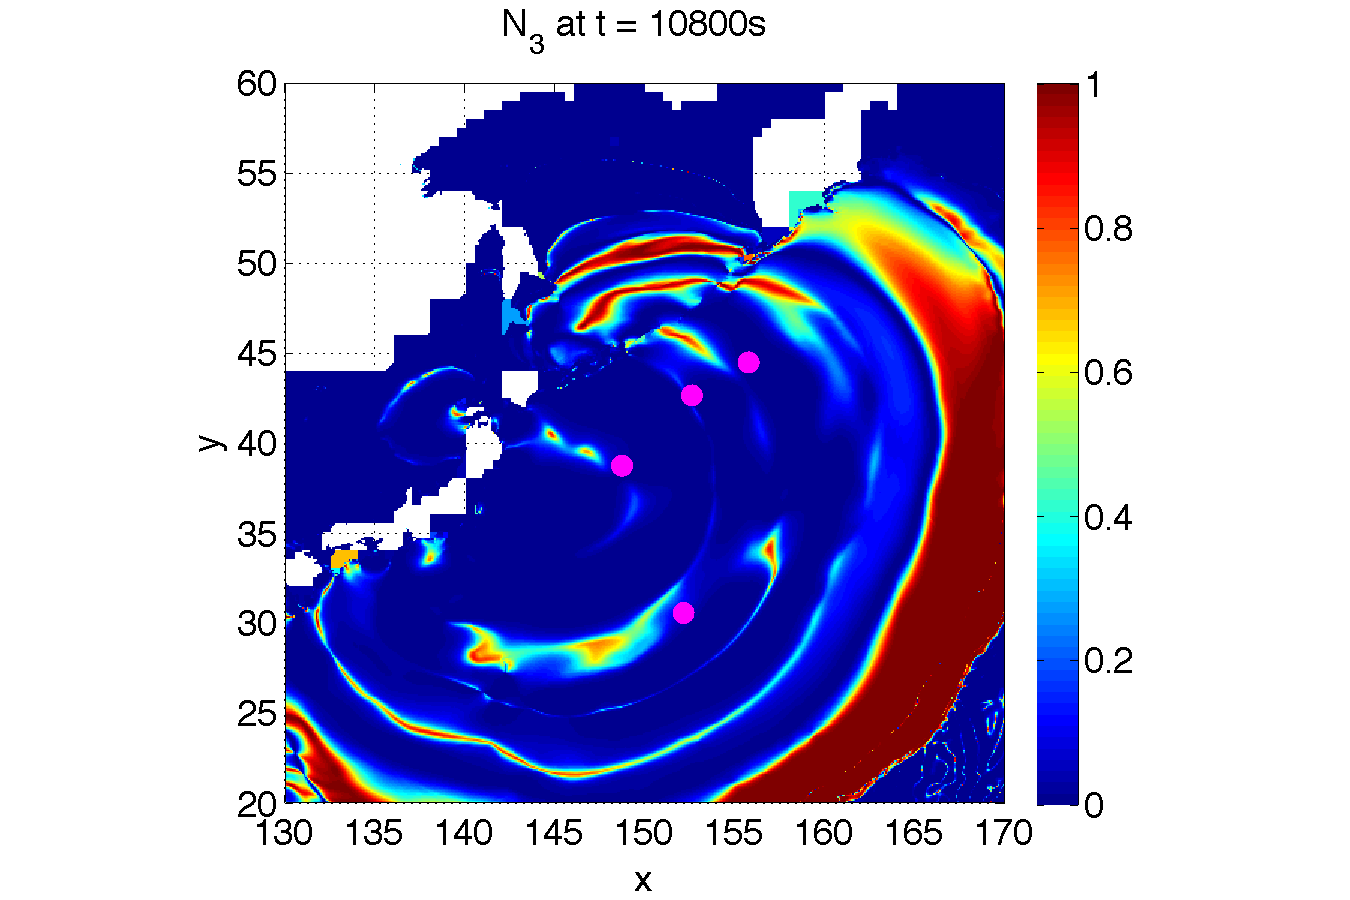
\includegraphics[width=0.45\textwidth]{../figures/T32d3.pdf} &
\hspace*{-65pt}
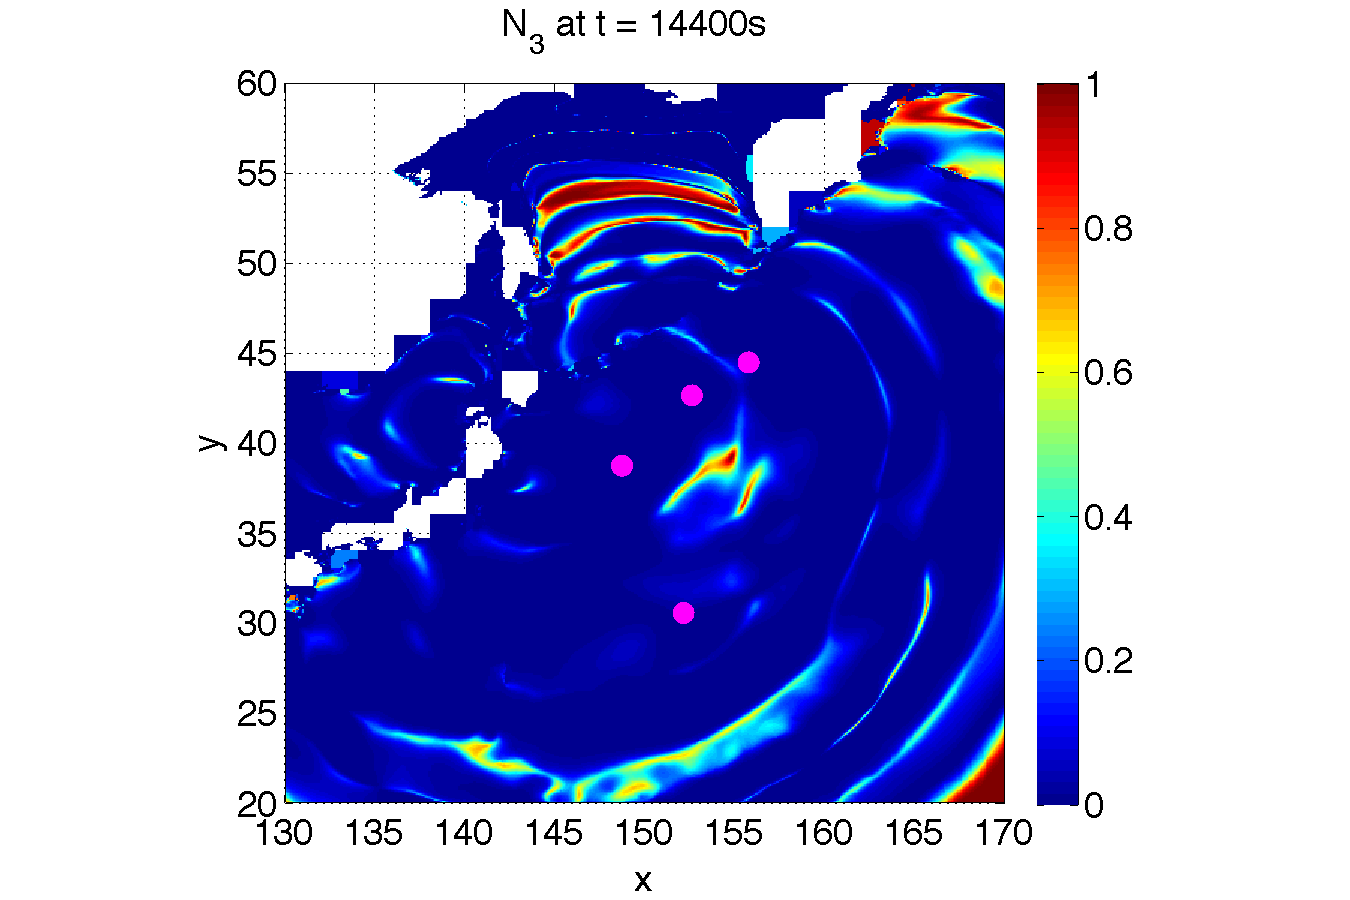
\includegraphics[width=0.45\textwidth]{../figures/T32d4.pdf}
\end{tabular}
\caption{Total sensitivity index for $N_1$ (top row) $N_2$ (center row) and $N_3$ (bottom row)
 at different times as indicated.}
\end{figure}
         
        
  \clearpage   